\section*{ODF Analysis}

\subsection*{Working with ODFs}

\begin{frame}
  \frametitle{Analyzing and Visualizing ODFs in \MTEX}

  \begin{center}
    \includegraphics[width=10cm]{latex_pic/odf2}
  \end{center}
\end{frame}

\subsection*{Working with ODFs}

\begin{frame}[fragile]
  \frametitle{Texture Characteristics}

Comparing {\bf arbitrary} ODFs
\begin{lstlisting}
calcerror(odf1,odf2,'L1')
\end{lstlisting}

\pause

Volume portions:
\begin{lstlisting}
volume(odf,center,radius)   % the volume of a ball
fibrevolume(odf,h,r,radius) % the volume of a fibre
\end{lstlisting}

\pause

Preferred orientations:
\begin{lstlisting}
q = modalorientation(odf) % the modal orientation
q = mean(odf)             % the mean orientation
\end{lstlisting}

\pause

The shape of the ODF:
\begin{lstlisting}
textureindex(odf)         % the texture index
entropy(odf)              % the entropy
fourier(odf,order)        % the C-coefficients
\end{lstlisting}


\end{frame}


\subsection*{Plotting (Inverse) Pole Figures}

\begin{frame}[fragile]
  \frametitle{Plotting (Inverse) Pole Figures in \MTEX}

  General syntax:
\begin{lstlisting}
plotpdf(odf,Miller(0,1,0),<options>)
plotipdf(odf,[xvector,zvector],<options>)
\end{lstlisting}

Options:
\begin{lstlisting}
antipodal % add antipodal symmetry
complete  % plot complete sphere
\end{lstlisting}


\onslide<1->
\center{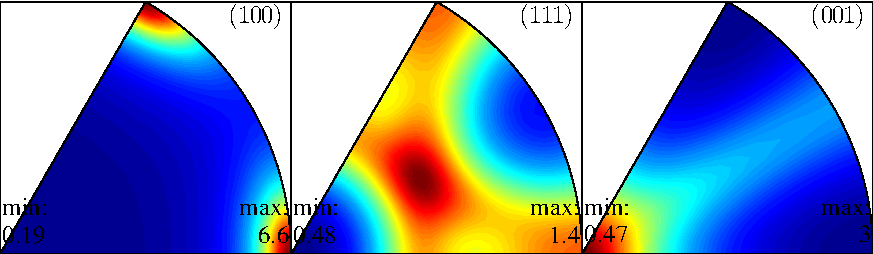
\includegraphics[height=3cm]{pic/ipdf}}

\end{frame}


\subsection*{Plotting an ODF}

\begin{frame}[fragile]
  \frametitle{Plotting  an ODF in \MTEX}

  \begin{columns}
    \begin{column}{6.5cm}
      General syntax:
\begin{lstlisting}
plot(odf,<options>)
\end{lstlisting}

      Sectioning:
      \lstset{emph={sigma},emphstyle={\color{blue}}}
\begin{lstlisting}
alpha, gamma, phi1, phi2
sigma, fibre
\end{lstlisting}

      Options:
\begin{lstlisting}
sections, center, resolution
\end{lstlisting}

      Example:
    \end{column}
    \begin{column}{5cm}
      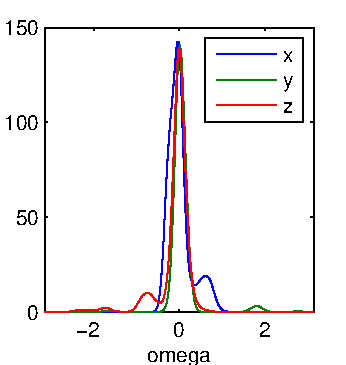
\includegraphics[width=5cm]{pic/radialplot}
    \end{column}
  \end{columns}

\begin{lstlisting}
plot(odf,'fibre',{Miller(0,0,1),zvector},...
  'center',modalorientation(odf))
\end{lstlisting}

%\begin{lstlisting}
%plot(odf,'alpha',[45*degree])
%\end{lstlisting}

\end{frame}


\subsection*{Dubna}

\begin{frame}[fragile]
  \frametitle{A Sigma Plot of the Recalculated Dubna ODF in \MTEX}

\begin{lstlisting}
plot(rec,'sections',18,'FontSize',10)
\end{lstlisting}

\medskip

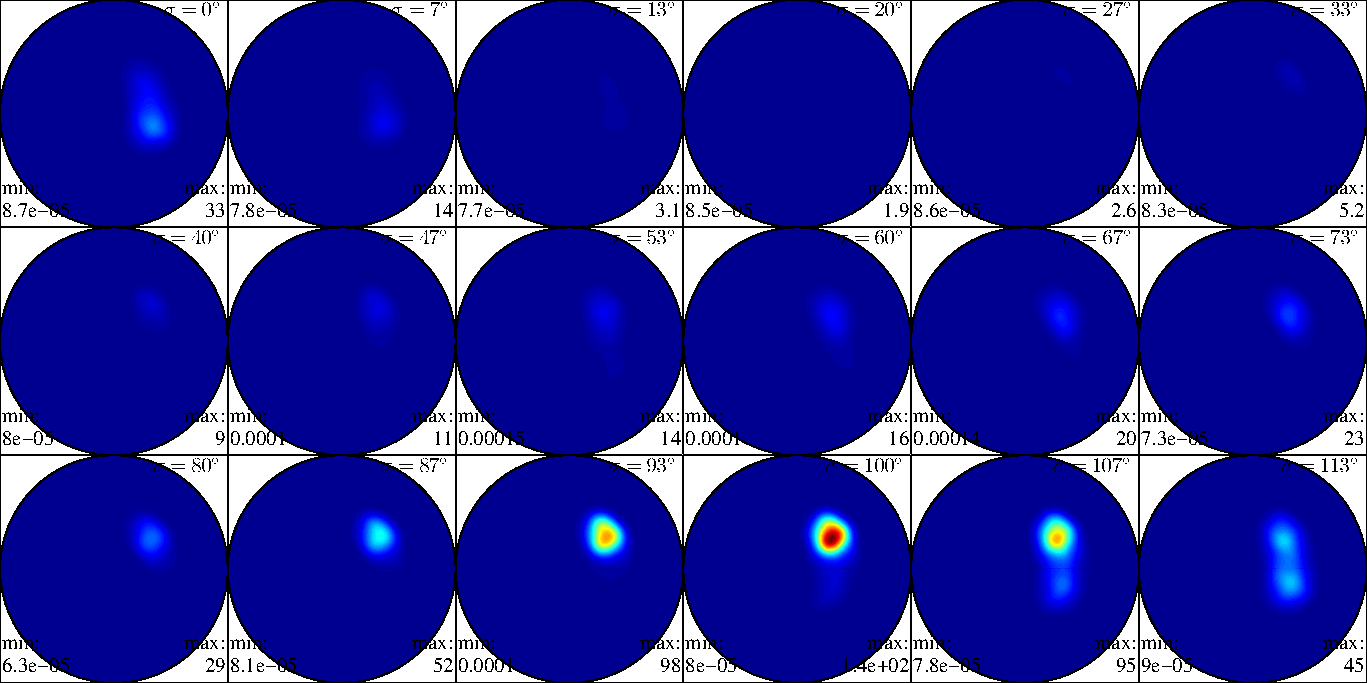
\includegraphics[width=\textwidth]{pic/ODFso9}

\end{frame}

\subsection*{Santafee}

\begin{frame}[fragile]
  \frametitle{The Classical Plot of the Santafee ODF in \MTEX}

\begin{lstlisting}
plot(santafee,'alpha','sections',18,...
     'projection','plain','gray','contourf')
\end{lstlisting}

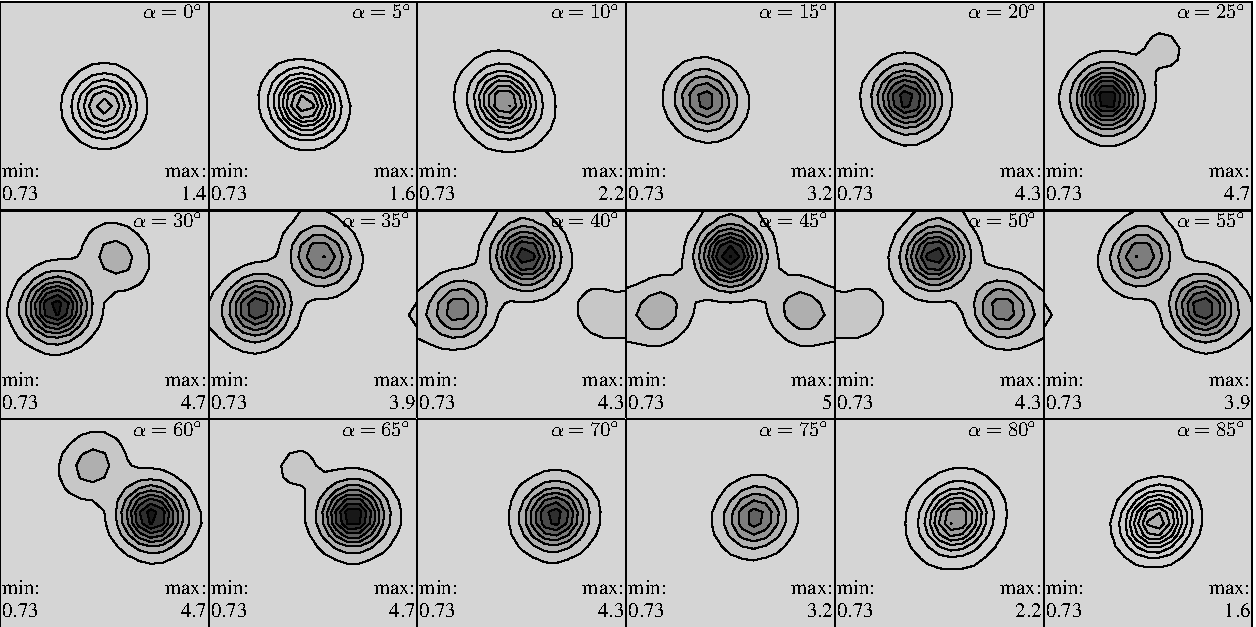
\includegraphics[width=\textwidth]{pic/santafee}

\end{frame}

\subsection*{Exercises}

\begin{frame}

  \begin{Exercise}
    \begin{enumerate}[a)]
      \item Construct a cubic unimodal ODF with mod at $[0 0 1](3 1 0)$.
      \item What is its modal orientation in Euler angles?
      \item Plot some pole figures. Are there pole figures that with and without
        antipodal symmetry? What about the inverse pole figures?
      \item Plot the ODF in $\sigma$ and $\phi_{2}$ - sections. How many mods
        do you observe?
      \item Compute the volume of the ODF that is within a distance of 10
        degree of the mod. Compare to an the uniform ODF.
    \end{enumerate}
  \end{Exercise}

  \begin{Exercise}
    \begin{enumerate}[a)]
    \item Construct a trigonal ODF that consists of two fibres at
      $h_1 = (0,0,0,1)$, $r_{1} = \vec y$, $h_2 = (1,0,\bar 1,0)$, $r_{2} = \vec x$.
    \item Do the two fibres intersect?
    \item What is the modal orientation of the ODF?
    \item Plot the ODF in $\sigma$ and $\phi_{2}$ - sections. How many
      fibre do you observe?
    \item Compute the texture index of the ODF.
    \end{enumerate}
  \end{Exercise}

\end{frame}


%%% Local Variables:
%%% mode: latex
%%% TeX-master: "main"
%%% End:
